%--------------------------------------%
%----- 3_Versuchsdurchführung.tex -----%
%--------------------------------------%
%--------------------------------------%
%
\subsection{Messung}
\label{subsec:3_Messung}
%
%------------------------------%
%----- Beginn eures Teils -----%
%------------------------------%
%
\begin{figure}[H]
  \Large
  \centering
  \begin{tikzpicture}[circuit ee IEC, font = \sffamily]
    \matrix(M)[
      matrix of nodes, nodes in empty cells,
      inner sep = 0pt, outer sep = -.1\pgflinewidth,
      column sep = 20mm, row sep = 15mm,
      nodes = {minimum width = 0pt}
      ]
    {
      & & & & & & & \\
      & & & & & & & \\
      & & & & & & & \\
      & & & & & & & \\
      & & & & & & & \\
      & & & & & & & \\
      & & & & & & & \\
      & & & & & & & \\
      & & & & & & & \\
    };
    %
    \draw[circuit symbol unit = 15pt]
      (M-4-2) to [sV] (M-6-2); 
    \draw[circuit symbol unit = 15pt]
      (M-2-4) to [capacitor = {info = $C_{1}$, info' = $\SI{1}{\nano\farad }$}] (M-4-4);
      \draw[circuit symbol unit = 15pt]
      (M-6-4) to [capacitor = {info = $C_{2}$, info' = $\SI{10}{\nano\farad }$}] (M-8-4);
    \draw[circuit symbol unit = 15pt]
      (M-4-4) to [resistor = {info = $R_{2}$, info' = $\SI{100}{\kilo\ohm}$}] (M-6-4);
    
    %
    \draw (M-2-2)--(M-4-2);
    \draw (M-6-2)--(M-8-2);
    \draw (M-2-2)--(M-2-4);
    \draw (M-8-2)--(M-8-4);
    \draw (M-4-4)--(M-4-6);
    \draw (M-8-4)--(M-8-6);
    
    \draw[fill=black] (M-4-4) circle (2pt);
    \draw[fill=black] (M-8-4) circle (2pt);
    \draw[fill=white] (M-4-6) circle (3pt);
    \draw[fill=white] (M-8-6) circle (3pt);
    
    %
    \draw[UPfeil = 6mm]
      ([xshift = -8mm]M-2-2.east)--([xshift = -8mm]M-8-2.east)
      node[midway, left]{$\underline{U}_\mathrm{E}$};
    \draw[UPfeil = 6mm]
      ([xshift = 0mm]M-4-6.east)--([xshift = 0mm]M-8-6.east)
      node[midway, right]{$\underline{U}_\mathrm{A}$};
    %\draw[IPfeil = 4mm]
    %  ([xshift = 3mm]M-2-2.center)--([xshift = 3mm]M-2-3.center)
      %node[midway, above]{$\underline{I}_\mathrm{}$};
    %
  \end{tikzpicture}
  \caption{Ersatzschaltbild des untersuchten Zweitors}
  \label{fig:schaltung}
\end{figure}
\subsubsection{Liste von Bauteile}:
\begin{itemize}
  \item Funktionsgenerator
  \item $100 \si{\kilo\ohm}$ Schichtwiderstand
  \item $1\si{\nano\farad}$ Kondensator
  \item 1 BNC-BNC Kabel
  \item $10 \si{\nano\farad}$ Kondensator
  \item 2 BNC-Doppelbananakabel
  \item Oszilloskop
  \item Steckbrett
\end{itemize}
\subsubsection{Ablauf}
Wir verbinden den $1\si{\nano\farad}$-Kondensator zunächst in Reihe mit dem Schichtwiderstand und mit dem 10nF-Kondensator. Der positive Pol der Quelle ist mit dem $1\si{\nano\farad}$-Kondensator auf dem Steckbrett und der negative mit dem $10 \si{\nano\farad}$ verbunden. Die Quelle ist auch parallel zu unserer gesamten Schaltung geschaltet. Das Oszilloskop wird parallel zum Widerstand und zum 10nF-Kondensatorzugang. Wir müssen jetzt mit dem Steckbrett auf unsere Quelle hören. Wir haben ein BNC-Doppelbananenkabel, dessen Stecker mit $V_a$ (positiver Pol) und $V_b$ (negativer Pol) verbunden sind. Jetzt müssen wir dasselbe mit dem Oszilloskop machen. Wir haben es mit dem Steckbrett durch ein BNC-Doppelbananenkabel durch $Vc$ (Pluspol) und Masse (Minuspol) gemacht. Wir müssen auch das Oszilloskop mit der Quelle verwalten. Hier haben wir ein BNC-BNC-Kabel.

Unsere Quelle sucht nach einem sinusförmigen Signal mit einer Spannung von 20 Volt von Spitze zu Spitze.

Wir müssen in unserem Versuch folgende Frequenzen betrachten:
$10,\dots,100$ (schritt:10)\\
$100,\dots,1000$ (schritt:100)\\
$1000,\dots,10000$ (schritt:1000)\\
$10000,\dots,100000$ (schritt:10000)\\
Wir haben dann $U_E$ am Channel 2 und $U_A$ am Channel 1.

In unserem Oszilloskop laufen wir mit dem Quellensignal und laufen zu horizontal/Frequenz und dann vertikal/$V_{pp}$, um die Frequenz und Spannung von $U_E$ zu messen. Wir wollen auch die Spannung von UA messen, also machen wir dasselbe für das gelbe Signal. Schließlich wollen wir den Zeitunterschied erkennen und zu horizontal/delay laufen.

Wir können jetzt anfangen zu messen. Wir notieren $U_{Epp}$, $U_{App}$, $f$ und $\Delta t$ auf.
%
%
%
\begin{flushright}
  \textit{\autorA}
\end{flushright}
%
%------------------------------%
%------ Ende eures Teils ------%
%------------------------------%
%
%
%
\subsection{Simulation}
\label{subsec:3_Simulation}
%
%------------------------------%
%----- Beginn eures Teils -----%
%------------------------------%
%
Für die Simulation wir bauen die Schaltung wie wir das im Experiment bauen, jedoch für $R_{mess}$, können wir für verschiedene Variabelen die gleiche Schaltung simulieren folgendes:
\begin{figure}[H]
  \centering
  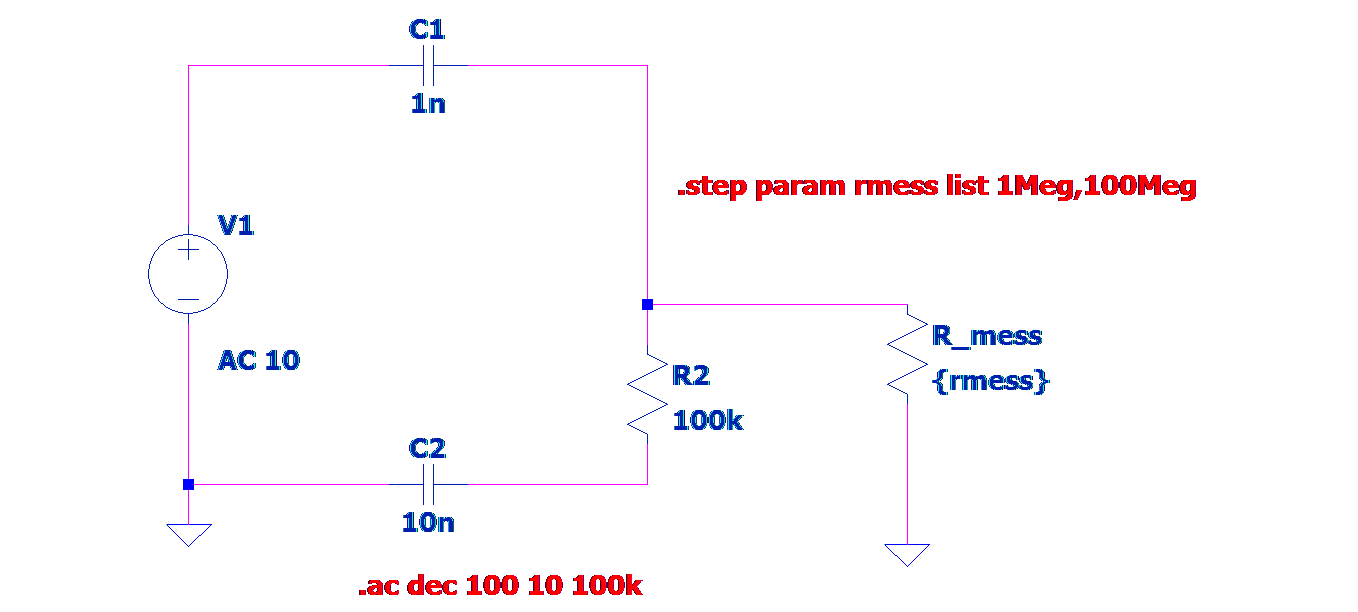
\includegraphics[scale=.4]{src/ltspice2.png}
  \caption{LTSpice schaltung}
  \label{fig:Schaltung von LTSpice}
\end{figure}
%
In den simulation, können wir SPICE befehlen schreiben, sodass wir verschiedene $R_{mess}$ gleichzeitig simulieren können.
\begin{figure}[H]
  \centering
  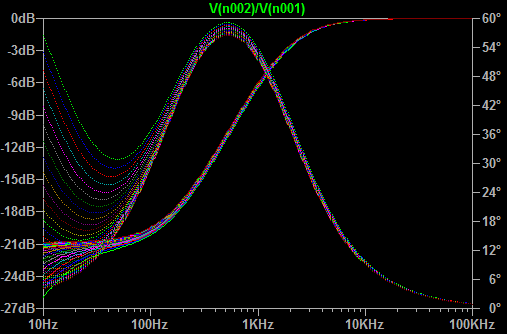
\includegraphics[scale=1]{src/ltspice5.png}
  \caption{Simulation in LTSpice}
  \label{fig:LTSpice simulation}
\end{figure}
%
%
\begin{flushright}
  \textit{\autorA}
\end{flushright}
%
%------------------------------%
%------ Ende eures Teils ------%
%------------------------------%
%
%
%